\section{Criptografia na computação}
\label{criptography}
Dentre as mudanças e impactos possíveis para a computação, a computação quântica possivelmente irá impactar diretamente a área de criptografia. Isso porque, os métodos criptográficos até então existentes podem ser quebrados através de estratégias de força bruta (que são algoritmos que buscam solução por tentativa e erro). Portanto, se o computador quântico pode executar diversas tarefas de forma exponencial, então, tais métodos criptográficos atuais se tornam obsoletos, o que gera um impacto direto na sociedade digital.

Todas as transações bancárias, correspondência civil e militar, diagnósticos médicos, votos em democracias, todas as formas de interação social que demandam alguma política de privacidade (por menor que sejam) serão afetadas. Portanto a computação quântica pode acirrar mais ainda o paradigma das questões privadas e sociais.

Esse capítulo apresenta uma introdução à área de criptografia, a fim de exemplificar em que premissas toda área repousa, por isso, será apresentada a estratégia de criptografia utilizando chaves pública-privada.

Conforme definido por Bruce Schneier \textit{``The art and science of keeping messages secure is cryptography […].''} \cite{13} Embora a criptografia seja considerada fundamental em nossas vidas digitais, ela não está especificamente relacionada à computação. A criptografia existe há milênios.

Na segurança cibernética, há uma série de preocupações quando se trata de dados. Isso inclui confidencialidade, integridade, disponibilidade e não repúdio.

\textbf{A confidencialidade} significa que nossos dados não podem ser acessados / lidos por usuários não autorizados.

\textbf{A integridade} do dado diz respeito à originalidade com a qual os dados chegam a nós, estando 100\% intactos, sem terem sido modificados – seja por um ato malicioso, perda de dados ou por algum outro fator. 

\textbf{A disponibilidade} se refere à acessibilidade dos dados quando necessário.

Examinaremos as várias formas de criptografia digital e como elas podem nos ajudar a alcançar os três objetivos listados acima. Quando falamos de criptografia digital, geralmente nos referimos aos conceitos abaixo, que serão especificados.

\begin{enumerate}
  \item Criptografia simétrica
  \item Criptografia assimétrica
  \item Funções de hash
\end{enumerate}

Temos receio que os computadores quânticos sejam capazes de decifrar certos códigos usados para enviar mensagens seguras. Esses códigos criptografam dados usando funções matemáticas de ``trapdoor'' que funcionam facilmente em uma direção, mas não em outra. Isso facilita a criptografia de dados, mas a decodificação é extremamente difícil sem a ajuda de uma chave especial.

Esses sistemas de criptografia não são inquebráveis e sua segurança se baseia na enorme quantidade de tempo que um computador clássico levaria para fazer o trabalho. Os métodos modernos de criptografia são projetados para que a decodificação demore tanto tempo que se tornem praticamente inquebráveis.

A chegada dos computadores quânticos mudou esse pensamento. Essas máquinas são muito mais poderosas que os computadores clássicos, tornando possível o rompimento desses códigos com facilidade, já que realizam contas matemáticas de forma mais eficiente e significativamente mais rápida que os computadores clássicos.

\subsection{Conceitos básicos de criptografia}
Antes de mergulharmos no conceito de criptografia, precisamos saber o que exatamente ela significa. Criptografar uma mensagem significa torná-la ilegível para partes não autorizadas usando uma cifra (o método específico para fazer isso). Descriptografar a mensagem significa reverter o processo e tornar os dados legíveis, decifrando-os mais uma vez.

\subsubsection{Criptografia simétrica}
Para criptografar e descriptografar corretamente nossos dados, precisamos de uma chave (que determina a saída da nossa cifra).  Na criptografia simétrica,  a chave usada para criptografar e decifrar os dados é a mesma, o que pode constituir em um problema de segurança. De forma a compreender este problema, pode-se refletir sobre como enviar dados com segurança em um ambiente hostil como a Internet. Nesse caso, se a mesma chave for usada para criptografar e decifrar dados, primeiro precisaríamos  enviar  a  chave  de  descriptografia  para  estabelecer  uma  conexão segura.  Porém, isso significa que estaríamos enviando a chave por uma conexão insegura, e assim ela poderia ser interceptada e usada por terceiros, se constituindo em um grande problema de segurança. 


\subsubsection{Criptografia assimétrica}
A criptografia assimétrica surge para resolver o problema da simétrica, possibilitando uma forma segura de compartilhamento de dados.

Para exemplificar esse novo formato, usaremos um cadeado que possui três estados – A (bloqueado), B (desbloqueado) e C (bloqueado) – E duas chaves distintas – A primeira pode girar apenas no sentido horário (de A a B a C) e a segunda pode girar apenas no sentido anti-horário (de C a B a A).

\vspace{1cm}
\begin{figure}[H] \centering 
  \makebox[\textwidth][c]{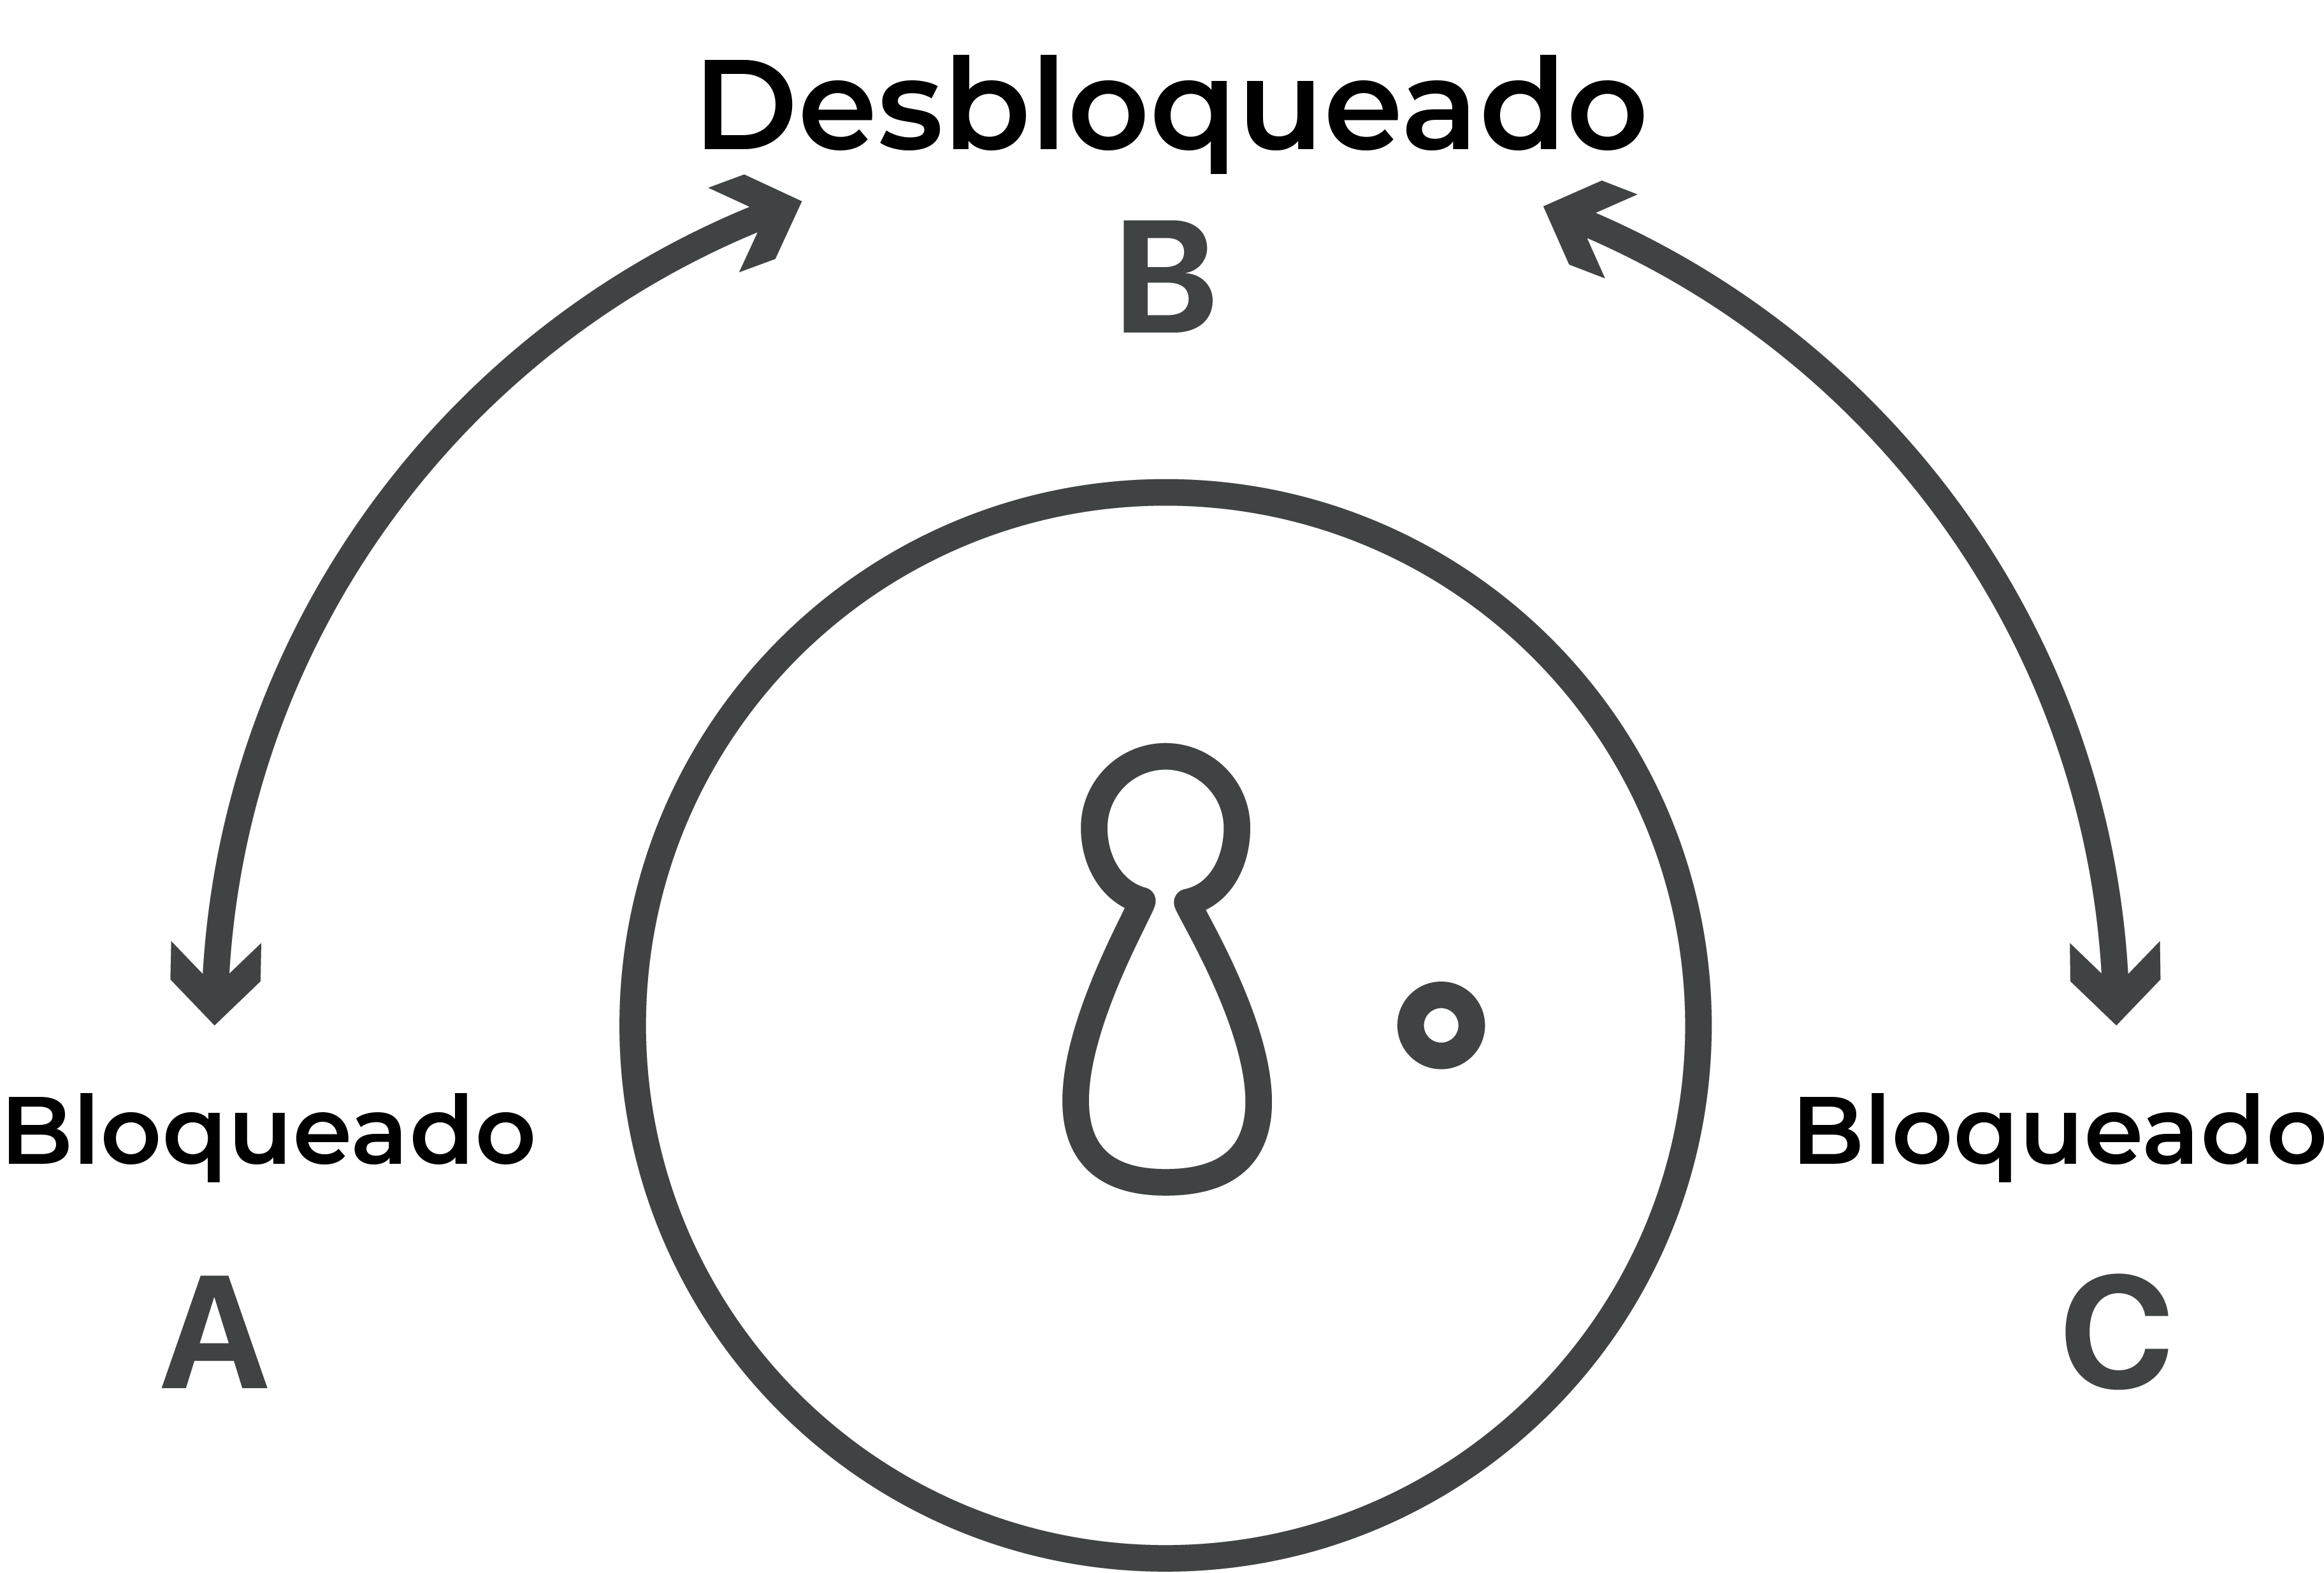
\includegraphics[width=0.8\textwidth]{cripto_keys}}
  \caption{\label{fig:5} Ilustração da posição das chaves} 
\end{figure}

Ao criptografar uma mensagem, o usuário pega a primeira chave e guarda para si mesmo. Essa chave é sua chave ``privada'' - porque apenas ele a possui.

A segunda chave é sua chave ``pública'': Pode ser distribuída para qualquer pessoa. Assim, o usuário tem sua chave privada que pode mudar de A para B para C. E todo os outros tem sua chave pública que pode mudar de C para B para A.

Colocando isso em prática, imagine que você queira enviar um documento privado para o usuário. Você coloca o documento na caixa e usa uma cópia da chave pública dele para bloqueá-lo. Lembre-se de que a chave pública dele gira apenas no sentido anti-horário, e você a coloca na posição A. Agora a caixa está bloqueada. A única chave que pode passar de A para B é a chave privada, a que ele guardou para si.

\subsubsection{Funções de hash}
Uma função de hash, diferentemente da criptografia simétrica / assimétrica, é  uma função unidirecional.  Você  pode criar um hash a partir de alguns dados, mas não há como reverter o processo. Portanto não sendo considerado uma maneira útil de armazenar dados, mas sim para verificar a integridade dos mesmos.  Uma função de hash recebe alguns dados como entrada e gera uma string aparentemente aleatória (mas nem tanto) que sempre terá o mesmo comprimento. Uma função de hash ideal cria valores exclusivos para diferentes entradas. A mesma entrada exata sempre produzirá exatamente o mesmo hash - e é por isso que podemos usá-la para verificar a integridade dos dados.

\subsection{Criando chave publica e privada RSA – Rivest Shamir Adleman}

De forma a aprofundar o conceito de criptografia assimétrica, foi criado um \href{https://github.com/gzsig/ic/tree/master/criptografia}{programa em linguagem C} que utiliza o algoritmo RSA\footnote{ Principal algoritmo de criptografia usado até os dias atuais, criado por Ron Rivest, Adi Shamire Leonard Adleman em 1977.}. O programa tem como objetivo apresentar de forma didática e visual o processo da execução do algoritmo RSA, gerando um par de chaves – pública e privada – e realizando o processo de criptografar e decifrar uma mensagem. A tabela \ref{criptography_step_by_step} a baixo ilustra esse processo.

\vspace{1cm}
\begin{longtable}{ |p{6cm}|| p{8cm}|  }
  \hline
  \multicolumn{2}{|c|}{RSA – Cryptosystem} \\
  \hline
    Descrição & matemática\\
  \hline
    Escolher dois números primos & 
    \[p=2\] \[q=7\]\\
  \hline
    Produto dos números escolhidos & 
    \[n=14\]\\
  \hline
    função Phi 
    \[\Phi(n)=(p-1)(q-1)\] & 
    \[\Phi(14)=(7-1)(2-1)\]
    \[\Phi(14)=(6)(1)\]
    \[\Phi(14)=6\]
    \[Coprimos\: de\: 14:\: 1, 3, 5, 9, 11, 13\]\\
  \hline
    Escolher o numero e `encryption'
    \begin{itemize}
      \item $1 < e < \Phi(n)$
      \item $coprimo\: de: n\: e\: \Phi(n)$
    \end{itemize} &
    \[Coprimos\: de\: 14:\: 1, 3, 5, 9, 11, 13\]
    \[Coprimos\: de\: 6:\: 1, 5\]
    \[Menor\: que\: 6\: e\: coprimo\: de\: 14\: e\: de\: 6: 5\]
    \[e = 5\]\\
  \hline
    Chave publica & 
    \[(5, 14)\]\\
  \hline
  Escolher o numero d `decryption'
    \begin{itemize}
      \item $d * e (mod \Phi(n)) = 1$
    \end{itemize} & 
    \[d * 5 (mod 6) = 1\]
    \[5*d = 5, 10, 15, 20, 25 \dots 55\]
    \[5*1 (mod 6) = 5\]
    \[5*2 (mod 6) = 4\]
    \[5*3 (mod 6) = 3\]
    \[5*4 (mod 6) = 2\]
    \[5*5 (mod 6) = 1\]
    \[5*6 (mod 6) = 0\]
    \[ \dots \]
    \[5*11 (mod 6) = 1\] \\
  \hline
  Chave privada & 
  \[(11, 14)\]\\
  \hline
  \caption{Passo a passo para gerar par de chaves}
  \label{criptography_step_by_step}
\end{longtable}

\vspace{1cm}
\begin{longtable}{ |p{6cm}|| p{8cm}|  }
  \hline
  \multicolumn{2}{|c|}{RSA – Cryptosystem} \\
  \hline
    Descrição & matemática\\
  \hline
    Criptografar \newline
    Chave publica: $(5, 14)$ \newline
    mensagem: ``B'' 
    \[A \to 1\]
    \[B \to 2\]
    \[C \to 3\]
    \[D \to 4\] & 
    \[2^5(mod 14)\]
    \[32(mod 14)\]
    \[4(mod 14)\]
    Mensagem criptografada: 4 $\to$ D\\
  \hline
    Decifrar \newline
    Chave privada: $(11, 14)$ \newline
    mensagem: ``D'' 
    \[A \to 1\]
    \[B \to 2\]
    \[C \to 3\]
    \[D \to 4\] & 
    \[4^{11}(mod 14)\]
    \[4194304(mod 14)\]
    \[2(mod 14)\]
    Mensagem original: 2 $\to$ B\\
  \hline
  \caption{Como criptografar e decifrar}
  \label{table:4}
\end{longtable}

\subsection{Criptografia aplicada computação clássica}
\subsection{Criptografia aplicada computação quântica}
\newpage

